\documentclass[10pt]{beamer}

\usepackage[english]{babel}
\usepackage[utf8]{inputenc}
\usepackage{amsmath,amssymb,amsthm,amscd,amsfonts}
\usepackage{xcolor}
\usepackage{graphicx}
%\usepackage{eulervm}
\usepackage{subfigure}
\usepackage{overpic}

\usepackage{epsfig}
\usepackage{color}

% Aspetto di beamer
\usetheme{CambridgeUS}
\usecolortheme{giove}

\setbeamertemplate{caption}{\raggedright\insertcaption\par}


\title[Splitting of homology of mapping class group]{Splitting of the homology of the punctured mapping class group}
\subtitle{Young Topologists Meeting, EPFL, Lausanne}
\author{Andrea Bianchi}
\date{26th July 2019}
\institute[Universit\"{a}t Bonn]{Mathematisches Institut, Universit\"{a}t Bonn}


\renewcommand{\epsilon}{\varepsilon}
\renewcommand{\phi}{\varphi}


\newcommand{\B}{\mathcal{B}}
\renewcommand{\P}{\mathcal{P}}
\newcommand{\ab}{\mathfrak{ab}}
\newcommand{\Sone}{\mathbb{S}^1}

\newcommand{\Z}{\mathbb{Z}}
\newcommand{\cF}{\mathcal{F}}
\renewcommand{\H}{\mathcal{H}}
\newcommand{\fM}{\mathfrak{M}}
\newcommand{\N}{\mathbb{N}}
\newcommand{\R}{\mathbb{R}}
\newcommand{\fS}{\mathfrak{S}}
\newcommand{\C}{\mathbb{C}}

\newcommand{\D}{\mathcal{D}}
\renewcommand{\S}{\mathcal{S}}
\newcommand{\sg}{\Sigma_{g,1}}
\renewcommand{\gg}{\Gamma_{g,1}}
\newcommand{\ggm}{\Gamma_{g,1}^m}
\newcommand{\Cb}{C_{\bullet}}


\newcommand{\set}[1]{\left\{#1\right\}}
\newcommand{\abs}[1]{\left|#1\right|}
\newcommand{\pa}[1]{\left(#1\right)}

\DeclareMathOperator{\Diff}{Diff}
\DeclareMathOperator{\Sym}{Sym}
\DeclareMathOperator{\Sp}{Sp}

\begin{document}

\maketitle

\begin{frame}{Configuration spaces of surfaces}
$\S:=\sg$ is an orientable surface of genus $g$ with one boundary
component.

\pause
The \emph{ordered} configuration space of $m$ points on $\S$ is
\[
 F_m(\S)=\set{(p_1,\dots,p_m)\in \mathrm{Int}(\S)^m \, | \, p_i\neq p_j \,\forall i\neq j}.
\]
\pause
The \emph{unordered} configuration space of $m$ points on $\S$ is
\[
 C_m(\S)=F_m(\S)/\fS_m.
\]
\pause
\vspace{-0.5cm}
\begin{figure}[h]
\subfigure{
\includegraphics[width=3cm]{ordered.pdf}
}
\hspace{1cm}
\subfigure{
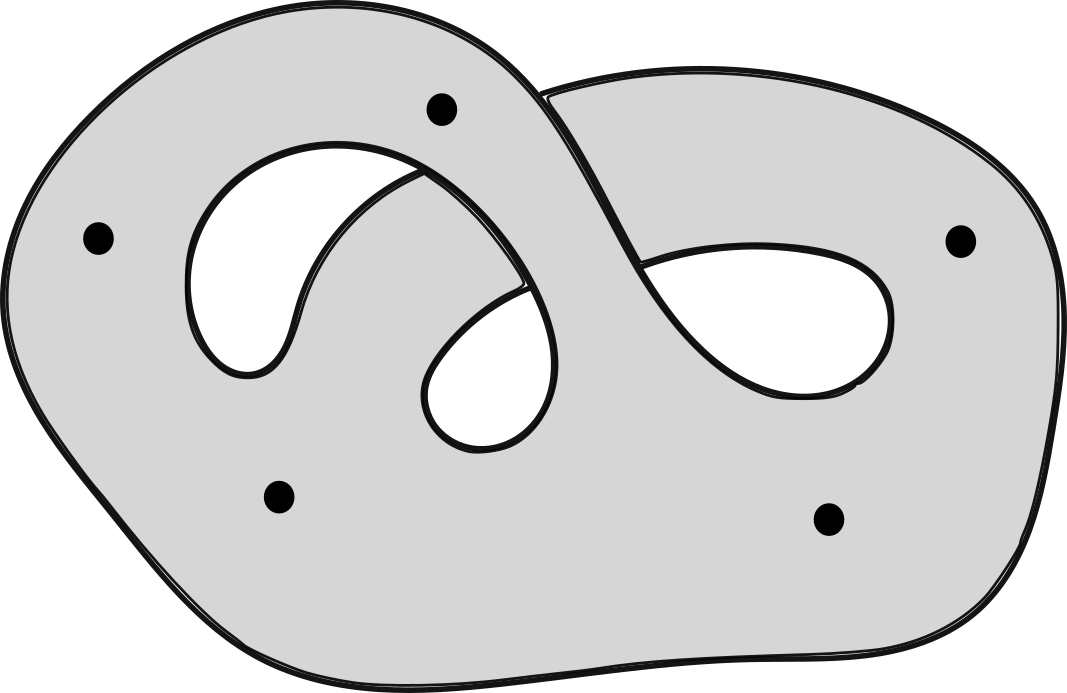
\includegraphics[width=3cm]{unordered.pdf}
}
\caption{A configuration in $F_5(\Sigma_{1,1})$ and the corresponding configuration in $C_5(\Sigma_{1,1})$.}
\end{figure}
\pause
\vspace{-0.5cm}
Want to compute $H_*(C_m(\S);\Z_2)$. From now on $H_*(-):=H_*(-;\Z_2)$. 
\end{frame}

\begin{frame}{Pontryagin rings and modules}
$\D:=\Sigma_{0,1}$ is the disc. Have product
$\mu\colon C_p(\D)\times C_q(\D)\to C_{p+q}(\D)$.
\begin{figure}[h]
\includegraphics[width=8cm]{product.pdf}
\end{figure}
\vspace{-0.3cm}
$\Cb(\D):=\coprod_{m\geq 0}C_m(\D)$ is (homotopy associative) $H$-space.
\pause

\vspace{0.1cm}
Fix $\D\hookrightarrow\S$ near $\partial\S$, and identify $\S\cong\S\setminus\D$. Have product
$\mu\colon C_p(\D)\times C_q(\textcolor{red}{\S})\cong C_p(\D)\times C_q(\textcolor{red}{\S\setminus\D})\to C_{p+q}(\S)$.
\begin{figure}[h]
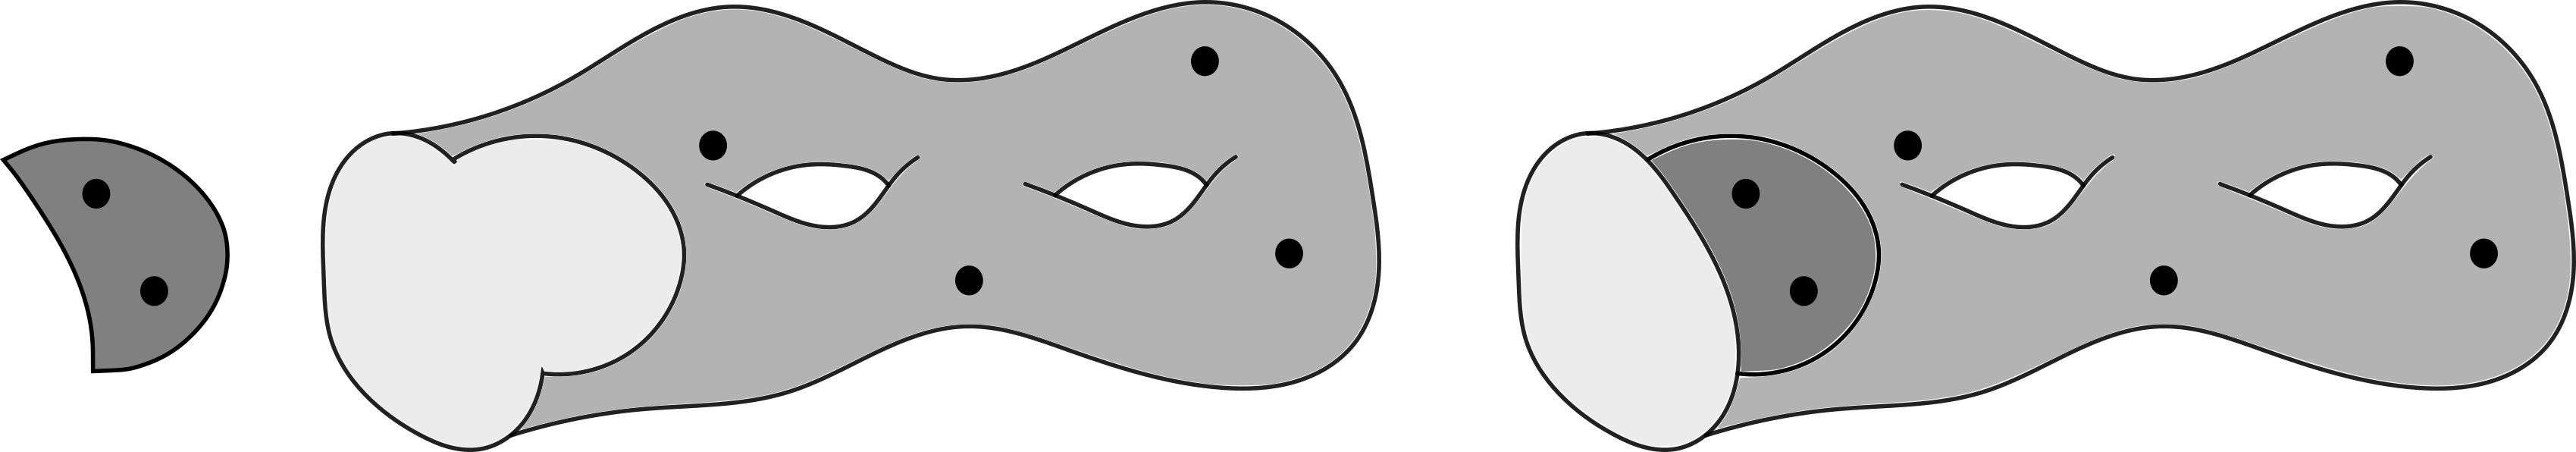
\includegraphics[width=9cm]{defmu.pdf}
\end{figure}
\vspace{-0.3cm}
$\Cb(\S):=\coprod_{m\geq 0} C_m(\S)$ is (homotopy assoc.) module over $\Cb(\D)$.

\pause
\vspace{0.1cm}
Then $H_*(\Cb(\D))=\bigoplus_{m\geq 0}H_*(C_m(\D))$ is a ring and $H_*(\Cb(\S))=\bigoplus_{m\geq 0}H_*(C_m(\S))$
is a $H_*(\Cb(\D))$-module.
\end{frame}


\begin{frame}{Mapping class group}
Recall $\D\hookrightarrow\S$ near $\partial \S$. $\Diff(\S)$ is the group of
diffeomorphisms $f\colon\S\to\S$ fixing $\textcolor{red}{\partial\S\cup\D}$ pointwise.
The \emph{mapping class group} is $\gg:=\Diff(\S)/$isotopy.

\pause
\vspace{0.1cm}
For all $m\geq 0$, $\Diff(\S)$ acts on $C_m(\S)$, hence $\gg$ acts on $H_*(C_m(\S))$.

\pause
Since $\D$ is fixed by all $f\in\Diff(\S)$, the action of $\gg$ on $H_*(\Cb(\S))$ is compatible
with the action of $H_*(\Cb(\D))$ on $H_*(\Cb(\S))$.
\pause
\begin{figure}[h]
\includegraphics[scale=0.5]{mappingclass.pdf}
\vspace{1mm}
\includegraphics[scale=0.5]{DiffactionCm.pdf}
\caption{A diffeomorphism $f$ acts on the product of two configurations in $C_3(\D)$ and $C_6(\S)$.}
\end{figure}

\pause
\vspace{-0.3cm}
Want to compute $H_*(\Cb(\S))$ as a $\gg$-representation in $H_*(\Cb(\D))$-modules.
\end{frame}




\begin{frame}{First result}
Let $\H:=H_1(\S)\cong H_1(C_1(\S))\simeq\Z_2^{2g}$.
\begin{block}{Theorem A (B.'19)}
There is an isomorphism of $\gg$-representation over $H_*(\Cb(\D))$
\[
 H_*(\Cb(\S))\cong H_*(\Cb(\D))\otimes_{\Z_2}\Sym_{\bullet}(\H).
\]
$\gg$ acts trivially on $H_*(\Cb(\D))$ and \emph{symplectically} on $\Sym_{\bullet}(\H)$.
\end{block}

\pause
Recall: the action of $\gg$ on $\H$ gives a surjective homomorphism $\gg\to\Sp_{2g}(\Z_2)$.
The action of $\gg$ on $H_*(\Cb(\S))$ is \emph{symplectic}, i.e. it
factors through the group $\Sp_{2g}(\Z_2)$.

\pause
\vspace{0.2cm}
\textbf{L\"offler-Milgram '88}. $H_*(\Cb(\S))$ is a \emph{symplectic} representation of $\gg$.

\textbf{B\"odigheimer-Cohen-Taylor '89}. Have isomorphism of \emph{bigraded} $\Z_2$-vector spaces.

\textbf{Cohen '76}. $H_*(\Cb(\D))\cong\Z_2[Q^j\epsilon|j\geq 0]$ as bigraded rings, with $Q^j\epsilon$
generator of $H_{2^j-1}(C_{2^j}(\D))\simeq\Z_2$.
\end{frame}

\begin{frame}{Examples of homology classes}
Here are some homology classes in $H_*(\Cb(\D))$: $\epsilon\in H_0(C_1(\D))$, $Q\epsilon\in H_1(C_2(\D))$, $Q^2\epsilon\in H_3(C_4(\D))$,
$\epsilon^3\cdot (Q\epsilon)^2\cdot Q^2\epsilon\in H_5(C_{11}(\D))$.

\begin{figure}[h]
\includegraphics[scale=0.47]{Qje.pdf}
\end{figure}

\pause
By Theorem A, $H_m(C_m(\S))\cong \Sym_m(\H)$ for all $m\geq 0$.
\pause
Let $c_1,\dots,c_m$ be \emph{disjoint} simple closed curves
on $\S$. Then $c_1\times\dots\times c_m\subset C_m(\S)$ is an embedded torus,
and $[c_1\times\dots\times c_m]\in H_m(C_m(\S))$ corresponds to $[c_1]\cdot\dots\cdot[c_m]\in\Sym_m(\H)$.

\begin{figure}[h]
\includegraphics[scale=0.67]{torus.pdf}
\caption{Three curves $c_1,c_2,c_3$ on $\S$ and the corresponding torus $c_1\times c_2\times c_3\subset C_3(\S)$.}
\end{figure}
\end{frame}

\begin{frame}{More examples of homology classes}
If the curves $c_1,\dots,c_m$ are not disjoint, we can still associate to $[c_1]\cdot\dots\cdot[c_m]\in\Sym_m(\H)$
a class in $H_m(C_m(\S))$. Here is an example.
\begin{figure}[h]
\includegraphics[scale=0.7]{intersection.pdf}
\end{figure}
\pause
% $c_1\times c_2\not\subset C_2(\S)$, but $(c_1\times c_2)\setminus R\subset C_2(\S)$
$R\subset c_1\times c_2$
is the \emph{rectangle} where both points are in the shaded region. $(c_1\times c_2)\setminus R\subset C_2(\S)$. $\partial R=\gamma=2\gamma'=0$.
% Can close $(c_1\times c_2)\setminus R$ in $C_2(\S)$ with a M\"obius strip.
Get class in $H_2(C_2(\S))$.

It is represented by $\mathbb{T}^2\sharp\R P^2\subset C_2(\S)$, it corresponds to $[c_1]\cdot[c_2]\in\Sym_2(\H)$.

\pause
\vspace{0.2cm}
We can complicate the example. Here is $\epsilon^2\cdot Q\epsilon\otimes [c_1]\cdot[c_2]\cdot[c_3]\cdot[c_4]$.
\begin{figure}[h]
\includegraphics[scale=0.7]{complicate.pdf}
\end{figure}
\end{frame}

\begin{frame}{Second result}
Fix $P_1,\dots, P_m\in \mathrm{Int}(\S\setminus\D)$. $\Diff^m(\S)$ is the group of
diffeomorphisms of $\S$ fixing $\partial\S\cup\D$ pointwise 
and \emph{permuting} the set $\set{P_1,\dots, P_m}$.

The \emph{punctured mapping class group} is $\ggm:=\Diff^m(\S)/$isotopy.

\pause
The \emph{$m$-th braid group} of $\S$ is $\beta_m(\S)=\pi_1(C_m(\S))$.

\pause
\vspace{0.1cm}
Birman's short exact sequence relates these groups:
\[
 1\to\beta_m(\S)\to\ggm\to\gg\to 1.
\]

\pause
Want to compute $H_*(\ggm)$ using Leray-Serre spectral sequence
\[
 E(m)^2_{p,q}=H_p\pa{\gg;H_q\pa{\beta_m(\S)}} \Rightarrow H_{p+q}\pa{\ggm}.
\]
\pause
\begin{block}{Theorem B (B.'19)}
The previous spectral sequence collapses on the second page. For all $l\geq 0$
\[
 H_l\pa{\ggm}\cong \bigoplus_{p+q=l} H_p\pa{\gg;H_q\pa{\beta_m(\S)}}.
\]
\end{block}
\end{frame}

\begin{frame}{From groups to classifying spaces}
$B\gg$ is the classifying space of $\gg$.
% The space $B\Diff(\S)=E\Diff(\S)/\Diff(\S)$ is also a $K(\gg,1)$ space. Let
% $\cF(\S):=\S\times_{\Diff(\S)} E\Diff(\S)$.
Have universal $\S$-bundle
\[
\S\hookrightarrow  \cF \overset{\pi}{\to} B\gg.
\]

\pause
For all $m\geq 0$ can apply $C_m(-)$ fiberwise. Get bundle with fiber $C_m(\S)$
\[
 C_m(\S)\hookrightarrow C_m(\pi)\to B\gg
\]
\pause
The previous fiber bundle of aspherical spaces classifies Birman $1\to\beta_m(\S)\to\ggm\to\gg\to 1$.
In particular $C_m(\pi)\simeq B\ggm$.

\pause
The associated spectral sequence is again 
\[
E(m)^2_{p,q}=H_p\pa{B\gg;H_q\pa{C_m(\S)}} \Rightarrow H_{p+q}\pa{C_m(\pi)}.
\]
\pause
Can operate product $\mu\colon C_p(\D)\times C_q(\S)\to C_{p+q}(\S)$ \emph{fiberwise}: get product
\[
 \mu^{\pi}\colon C_p(\D)\times C_q(\pi)\to C_{p+q}(\pi)
\]
\pause
It is a map of bundles over $B\gg$. Get map of spectral sequences $\mu^{\pi}\colon H_*(C_p(\D))\otimes_{\Z_2} E(q)\to E(p+q)$.
Theorem B by induction.
\end{frame}

\begin{frame}{A convenient reformulation}
Let $\Cb(\pi):=\coprod_{m\geq 0} C_m(\pi)$, where
\[
 C_m(\S)\hookrightarrow C_m(\pi)\to B\gg.
\]
\pause
The extended products $ \mu^{\pi}\colon C_p(\D)\times C_q(\pi)\to C_{p+q}(\pi)$
 make $\Cb(\pi)$
into a $\Cb(\D)$-module.

\pause
\vspace{0.3cm}
Passing to homology, $H_*(\Cb(\pi))$ is a $H_*(\Cb(\D))$-module.

\pause
\begin{block}{Reformulation of Theorem B}
There is an isomorphism of $H_*(\Cb(\D))$-modules
\[
 \pa{\bigoplus_{m\geq 0}H_*(\ggm)\cong} H_*(\Cb(\pi))\cong H_*(\Cb(\D))\otimes_{\Z_2} H_*(\gg;\Sym_{\bullet}(\H)).
\]
\end{block}
\vspace{0.5cm}
\pause
\centering{\large{Thank you for your attention!}}


\end{frame}



\end{document}
